\chapter{実験}
ここでは、本研究の実験が行なった実験について述べる。

\section{予備実験}
ここでは、本研究が実験を行うにあたってその準備実験の試行として行なった実験について述べる.


%\subsection{データセット}
%この研究ではドライブレコーダーから得られる映像を用いて実験を行う。
%その際、データーセットとしてYouTube等の動画投稿サイトに投稿されたドライブレコーダーの動画を用いる。

\subsection{予備実験}
本研究ではドライブレコーダーから得られる動画を用いて実験、評価を行うが、その予備実験として動画から切り出された画像を用いて本研究のシステムの実験を行った。
この予備実験は、本研究を行うにあたって、距離推定プログラムあるいは深度推定プログラムの候補が2つあり、そのどちらが相応しいかを決める実験である。
その結果を\figref{fig:preex}とに示す。
\figref{fig:preex}のように、このシステムは画像を上下二段に切り分け、上段では入力された映像の高さを半分にした画像、下段はその画像を用いて奥行き推定を行ったものである。
また、上段で自動車とトラックを検出し、下段の同じ位置にBBOXを出力している。
下段のBBOX内に出力されているパラメーターは、下段BOX内のRGB値のそれぞれの値を平均した数値である。

\begin{figure}[htbp]
  \begin{minipage}{0.5\hsize}
   \begin{center}
    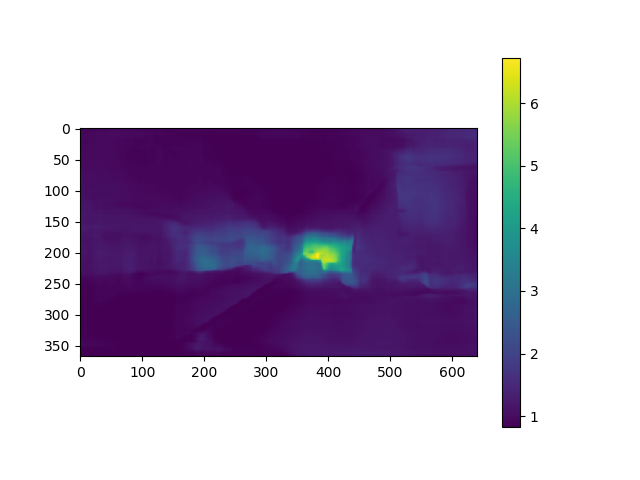
\includegraphics[width=7cm]{figs/preex1.png}
   \end{center}
   \caption{FCRN-DepthPredictionを用いた予備実験}
   \label{fig:preex1}
  \end{minipage}
  \begin{minipage}{0.5\hsize}
  \begin{center}
   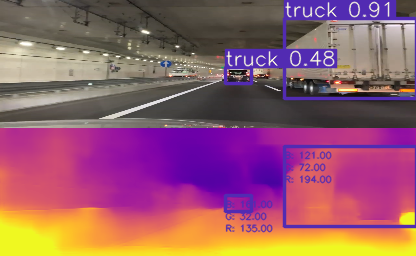
\includegraphics[width=7cm]{figs/preex2.png}
  \end{center}
   \caption{Google Tensorflowを用いた予備実験}
   \label{fig:preex2}
  \end{minipage}
 \end{figure}

\subsection{予備実験 - 評価}
ここでは、本研究における予備実験の評価について述べる。
\figref{fig:preex1}と\figref{fig:preex2}を比較すると、前者は深度推定を行なった結果のみを出力するのに対し、後者は元の画像を圧縮し上下二段二分けて出力されていることがわかる。
また、前者は奥にある物体が明るく色分けされているが、カメラから近いところにある道路やトラックなど、ほぼ暗い青色で塗り分けられているだけであり、物体の識別が難しい。
それに対して後者はカメラから近い距離にある物体ほど明るく塗り分けられており、奥にある物体ほど暗い色になっている。
前者と後者を比較した際、特に違いが顕著なのは後者のシステムの方が画面左側にあるトラックをはっきりと色分けできているという点である。
そのため、本研究においては後者のGoogle Tensorflowを採用し、本実験を行うことにする。

また、\figref{fig:preex2}を見ればわかる通り、物体検出システムと距離推定システムを用いることで先行車との大まかな車間距離を調べることが可能なことがわかる。
\figref{fig:preex2}においてシステムが検出した自動車をそれぞれ右から車1、車2とおくと、下段のRGB値のそれぞれの平均を見てみると、奥にある車1の方が手前にある車2よりもR,Gの値が低く、Bの値が高いことがわかる。
%距離推定システムは奥行きを手前にある物体ほど色を明るく、奥にある(カメラから距離が遠い)物体ほど暗い青色で色分けするので、このシステムで先行車の位置関係が大まかにわかることが確認できる。
この数値の違いを評価することで先行車との距離を推定し、走行スピードを推定し、渋滞しているかどうかを機械に判断させる。
この予備実験を生かして、本実験では動画を用いた渋滞推定を行う。